\usetikzlibrary{arrows}
\usetikzlibrary{positioning}


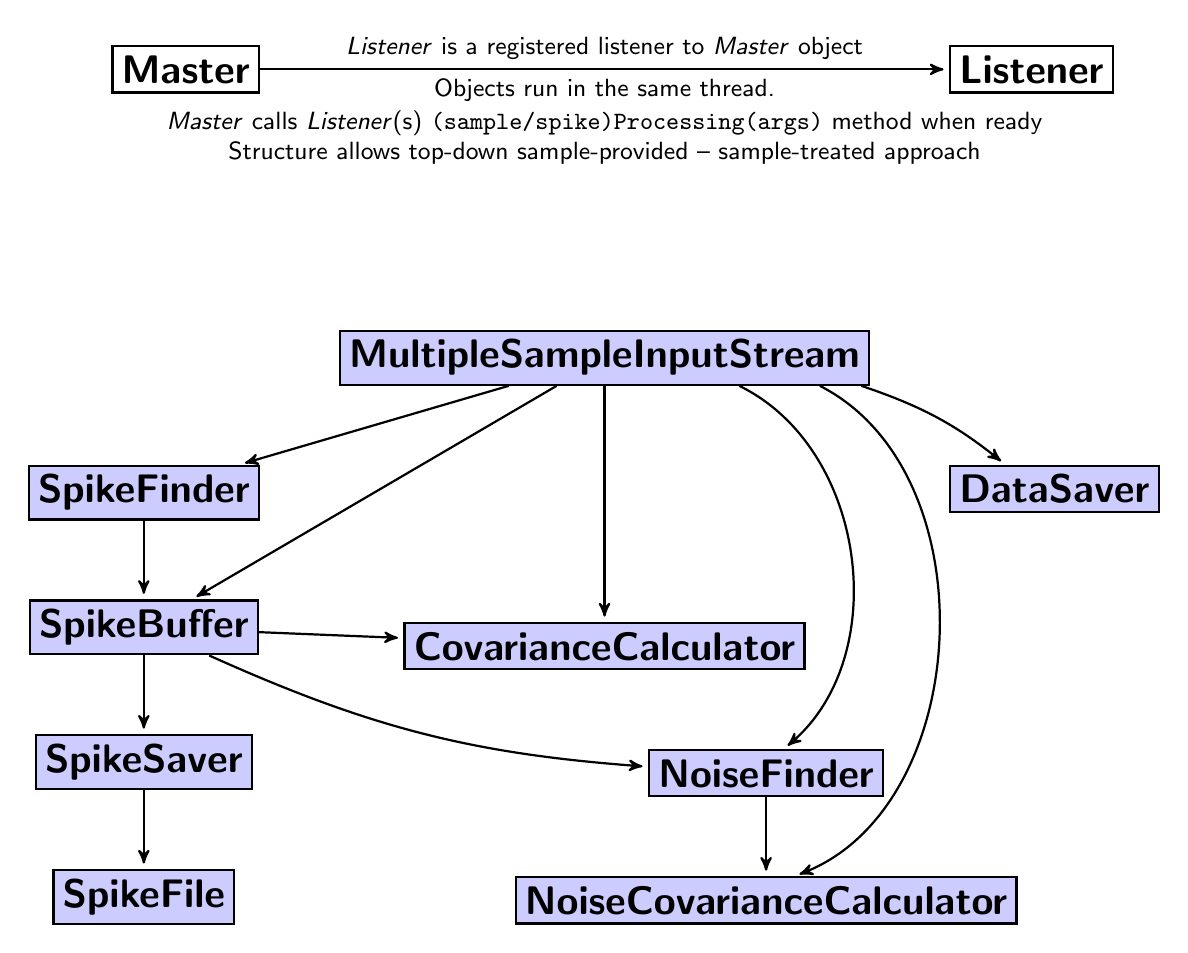
\begin{tikzpicture}[->,>=stealth',shorten >=2pt,auto,node distance=3cm,
  thick,main node/.style={rectangle,fill=blue!20,draw,font=\sffamily\Large\bfseries},
  legend node/.style={rectangle,draw,font=\sffamily\Large\bfseries}]


  \node[main node] (MSIF) {MultipleSampleInputStream};
  \node[main node] (SFnd) [below left = 1 and 1 of MSIF] {SpikeFinder};
  \node[main node] (SB) [below = 1 of SFnd] {SpikeBuffer};
  \node[main node] (CC) [below = 3 of MSIF] {CovarianceCalculator};
  \node[main node] (NF) [below right = 1 and -2 of CC] {NoiseFinder};
  \node[main node] (NCC) [below = 1 of NF] {NoiseCovarianceCalculator};
  \node[main node] (SS) [below = 1 of SB] {SpikeSaver};
  \node[main node] (SFl) [below = 1 of SS] {SpikeFile};
  \node[main node] (DS) [below right= 1 and 1 of MSIF] {DataSaver};
  \node[legend node] (Mst) [above left = 3 and 1 of MSIF] {Master};
  \node[legend node] (Lst) [above right = 3 and 1 of MSIF] {Listener};

    \tikzstyle{samplestyle} = [->,>=stealth',shorten >=2pt,auto]
\tikzstyle{spikestyle} = [double]

    
  \path[every node/.style={font=\sffamily\small}]
    (MSIF) edge node [left = 0.5] {} (SFnd)
         edge node [right = 0.3] {} (SB)
         edge node [left] {} (CC)
         edge [bend left = 57] node [left] {} (NF)
         edge [bend left = 66] node [right] {} (NCC)
         edge [bend left = 10] node [right] {} (DS)
    (SFnd) edge node [right] {} (SB)
    (SB) edge node [below] {} (CC)
         edge [bend right = 10] node [below] {} (NF)
         edge node [right] {} (SS)
    (NF) edge node [left]  {} (NCC)
    (SS) edge node [right] {} (SFl)
    (Mst) edge node [above] {\emph{Listener} is a registered listener to \emph{Master} object} 
    			node [below] {Objects run in the same thread.}
    			node [below = 0.4] {\emph{Master} calls \emph{Listener}(s) \texttt{(sample/spike)Processing(args)} method when ready}
    			node [below = 0.8] {Structure allows top-down sample-provided -- sample-treated approach} (Lst)
    			;
    			
\end{tikzpicture}


